\chapter{Das REST Architekturkonzept}
\section{Entstehung}
Das Architekturkonzept des Representational State Transfer wurde erstmals im Jahr 2000 von Roy T. Fielding erwähnt, definiert und mit dem Akronym REST bezeichnet.\cite[76]{REST}
Es enthält eine Reihe von Prinzipien für die Entwicklung von verteilten Systemen im Web mit besonderem Fokus auf den Schnittstellen zwischen den einzelnen Komponenten.
Dabei baut REST auf der Client-Server-Architektur auf und hatte durch die Arbeit vib Fielding in den HTTP- und URI-Arbeitsgruppen direkten Einfluss auf die Entwicklung von der beiden Standards, wodurch jene Schnittstellen im Web definiert werden.\cite[vgl.][4,105f.]{REST}
REST beschreibt größtenteils die Architektur des Web selbst und ist daher nicht auf APIs ausgelegt oder beschränkt\cite[vgl.][1]{Tilkov}.

\section{Grundlagen}
\subsubsection{Ziele von REST}
Die Ziele und Vorteile der REST Architektur lassen sich folgendermaßen zusammenfassen:
\foreignblockcquote{english}[105]{REST}{REST provides a set of architectural constraints that, when applied as a whole, emphasizes scalability of component interactions, generality of interfaces, independent deployment of components, and intermediary components to reduce interaction latency, enforce security, and encapsulate  legacy  systems.}
Diese Ziele werden erreicht durch eine Reihe von Anforderungen.
\subsubsection{Komponenten und Prinzipien}
Die REST Architektur baut auf der weit verbreiteten Client-Server Architektur auf und definiert den Begriff der Ressource als Abstraktion für jede Art von Information, die Ziel einer Client-Anfrage ist.\cite[vgl.][88f.]{REST}
Als Beispiele für Ressourcen nennt Fielding selbst: \textcquote[88]{REST}{a document or image, a temporal service [\dots], a collection of other resources, a non-virtual object (e.g.\ a person).}
Eine Ressource wird durch einen Bezeichner bekannt gemacht und ist damit für einen Client abrufbar.
Der Bezeichner bleibt gleich, selbst wenn sich die damit identifizierte Ressource ändert.
Die Kommunikation einer Ressource vom Server zum Client erfolgt über eine Repräsentation der Ressource, d.h.\ ein Datenformat, welches vom Server festgelegt oder durch Content-Negotiation zwischen Client und Server ausgehandelt wird.
Somit bleibt der Ursprung der Daten hinter der Serverschnittstelle versteckt.
Die Antwort des Servers enthält die Daten der Repräsentation und deren Metadaten.
Anfrage und Antwort enthalten außerdem Kontrolldaten, \zB{} HTTP Request Methods, Status Codes und Header, um die Bedeutung der Nachricht zu vermitteln.\cite[vgl.][90f.]{REST}
{\rowcolors{2}{white}{blue!30!white!70}
\begin{table}[h!]
  \begin{center}
    \caption{REST Data Elements, in Anlehnung an~\cite[88]{REST}}\label{tab:REST Data Elemens}
    \begin{tabularx}{\linewidth}{m{0.2\linewidth}m{0.33\linewidth}X}
      \rowcolor{blue!40!white!50!black!10}\textbf{Data Element} & \textbf{Web Equivalent} & \textbf{Example}\\
      \midrule
      resource & the intended conceptual target of a hypertext reference & a list of events\\
      resource identifier & URI & http://example.com/events\\
      representation data & HTML, JSON Document, PNG image & \{events:[\{id:4,title:\dots\},\{\dots\}]\}\\
      representation metadata & media type, last-modified time, ETag & Content-Type: application/json, Content-Encoding: gzip\\
      control data & if-modified-since, cache-control, request method & GET, Cache-Control: no-cache\\
    \end{tabularx}
  \end{center}
\end{table}
}
\par
REST ist zustandslos, sodass jede Anfrage vom Client zum Server alle für deren Verarbeitung notwendigen Informationen beinhalten muss.
Ein Client speichert gewöhnlich seinen Zustand, während auf Serverseite keine Zustandsinformationen über mehrere Anfragen hinweg gespeichert werden, wie es zum Beispiel bei Sessions der Fall ist.
Aufgrund dieser Eigenschaft wird im Zusammenhang mit REST auch von einer \foreigntextcquote{english}[83]{REST}{Client-Cache-Stateless-Server[-Architektur]} gesprochen.
Hieraus ergeben sich drei Vorteile:\cite[vgl.][79]{REST}
\begin{itemize}
  \item Sichtbarkeit:
  Jede Anfrage kann separat untersucht und gecacht werden, ohne weitere Informationen zu benötigen.
  \item Zuverlässigkeit:
  Anfragen können atomar betrachtet und bei Teilfehlern kann ein stabiler Systemzustand leicht wiederhergestellt werden.
  \item Skalierbarkeit:
  Da ein Server Zustandsinformationen nur für die Dauer der Verarbeitung einer Anfrage speichert, können Ressourcen schnell wieder freigegeben werden.
\end{itemize}
Nachteil dieser Anforderung ist eine verringerte Netzwerkperformance, da bei sequenziellen Anfragen an einen Server, Daten zur Clientidentifikation, Authentifizierung oder aus vorangegangene Antworten erneut gesendet werden müssen.
Die verringerte Kopplung führt ebenfalls dazu, dass die Kontrolle des Servers über das Verhalten der Clientanwendung reduziert wird.
\par
Clientseitiges Speichern von erhaltenen Daten (Caching) erlaubt die Wiederverwendung früherer Serverantworten für zukünftige, gleiche Anfragen und ist sinnvoll, da die gefühlte Performance durch Verringerung der durchschnittlichen Latenz erhöht wird.
Dadurch wird die Effizienz und Skalierbarkeit der Anwendung erhöht, obwohl die Latenz jeder einzelnen Anfrage durch den Cache-Lookup erhöht wird.
Je mehr die gespeicherten Daten von den tatsächlichen Daten abweichen, desto mehr verringert sich die Verlässlichkeit derselben.\cite[vgl.][80]{REST}
GET-Requests werden von Webbrowsern implizit gecacht, wobei Server das gewünschte Caching-Verhalten explizit erlauben und verbieten können.

REST beschreibt drei Typen von Komponenten:\cite[vgl.][96]{REST}
\begin{itemize}
  \item User Agent:
  Dies kann ein Webbrowser bzw.\ die Benutzeranwendung sein, in jedem Fall jedoch der letztendliche Empfänger der Antwort.
  \item Origin Server:
  Die endgültige Quelle der Repräsentation einer Ressource und der letztendliche Empfänger von Request, die zu Modifikationen der Daten führen.
  \item Intermediary (Zwischenkomponenten):
  Diese befinden sich zwischen User Agent und Origin Server und können sowohl als Client, als auch als Server agieren. Sie leiten Anfragen und Antworten weiter, können diese aber auch modifizieren. Je nach Anwendungsfall spricht man hier von einem Gateway oder Proxy.
\end{itemize}
Für die Schnittstellen der Komponenten gelten folgende Grundsätze:\cite[vgl.][82]{REST}
\begin{itemize}
  \item Ressourcen müssen durch einen Bezeichner eindeutig identifizierbar sein.
  Die URI für eine Ressource wird auch als Endpunkt bezeichnet.
  \item Die Interaktion mit einer Ressource, d.h.\ das Abfragen und Manipulieren derselben erfolgt über eine Repräsentation der Ressource.
  \item Nachrichten müssen so selbsterklärend sein, dass sie von der Schnittstelle verstanden und verarbeitet werden können.
  \item \foreigntextcquote{english}[82]{REST}{hypermedia as the engine of application state} (HATEOAS): Der Hypertext beschreibt den Zustand der Anwendung und die Möglichkeiten der Veränderung desselben.
  Folgt der Client einem Link im Hypertext und fordert eine neue Repräsentation an, so ändert er seinen Zustand.
  Dieses Prinzip ist daher auch namensgebend für die Architektur des Representational State Transfer~\cite[vgl.][103f.]{SOA}.
\end{itemize}
\par
Durch die generischen Client- und Serverschnittstellen, die selbstbeschreibenden Nachrichten und die zustandslose Kommunikation kann eine REST Anwendung leicht von Schichten profitieren.
Keine einzelne Komponente benötigt Kenntnis des gesamten Informationsweges, sondern sieht nur die Komponenten, mit denen sie direkt interagiert, sodass zwischen
User-Agent und Origin-Server Zwischenkomponenten eingeführt werden können, um spezifische Aufgaben, wie Caching, Kapselung, Load Balancing und Datentransformation, zu übernehmen.\cite[vgl.][99]{REST}
Die so verbesserte Skalierbarkeit des Servers bringt jedoch mehr Datenverarbeitung durch die Zwischenkomponenten und somit höhere Latenzzeiten mit sich.\cite[vgl.][83,98]{REST}
\begin{figure}[h]
  \centering
  \fbox{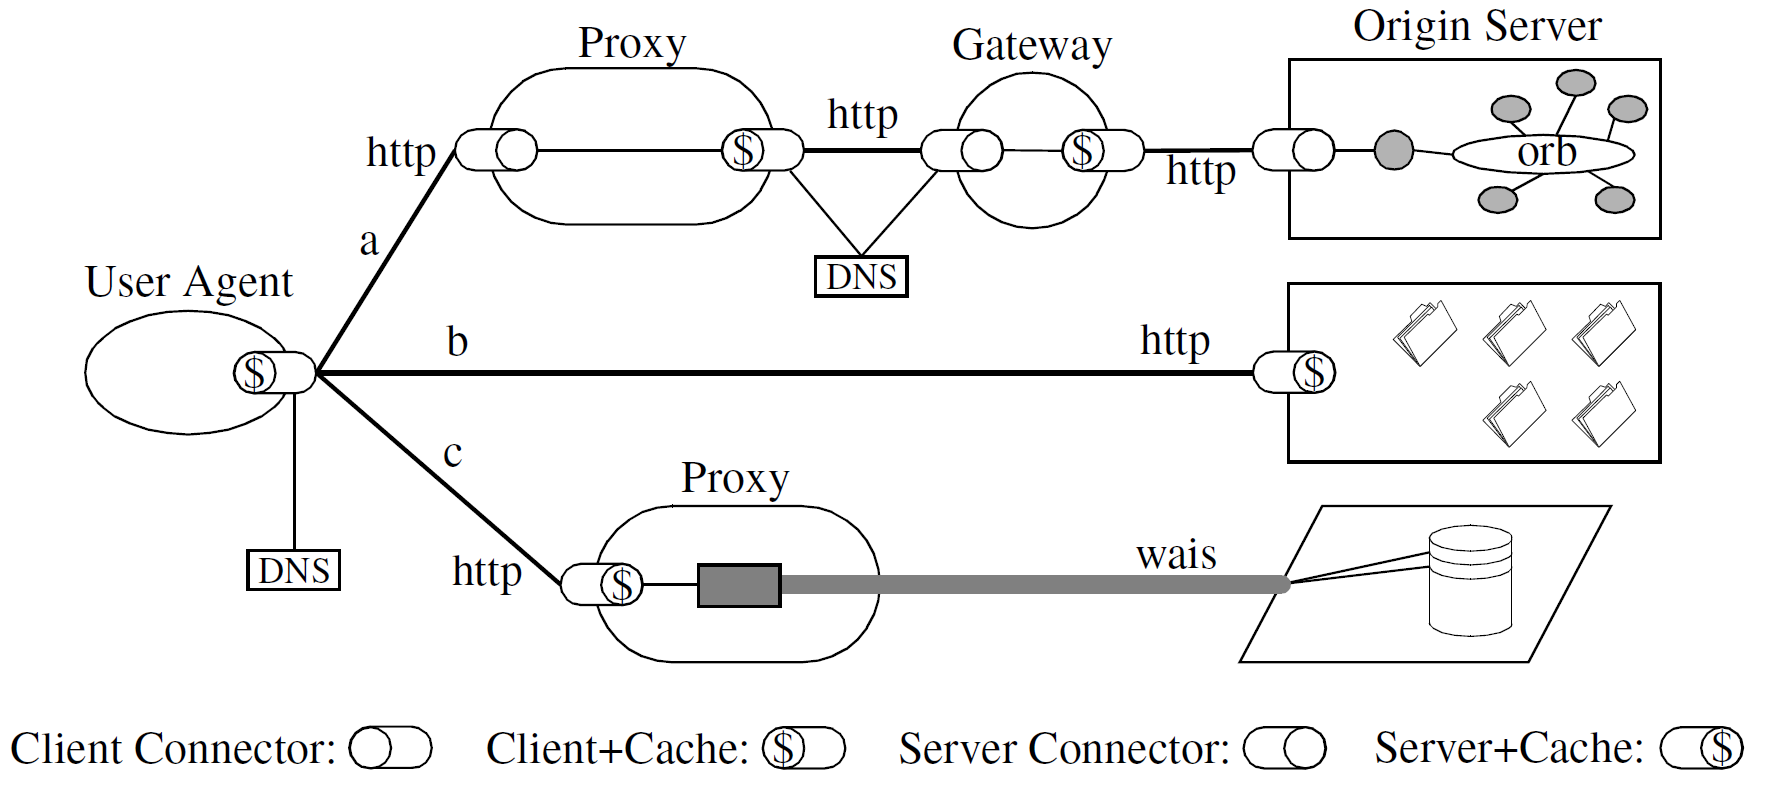
\includegraphics[width=\linewidth]{REST-process-view.png}}
  \caption{REST~\cite[84]{REST}}\label{img:REST-diss}
\end{figure}

\section{Implementierung von RESTful APIs}
Eine API, die dem REST Architekturstil folgt, wird RESTful genannt.
Da die Dissertation von Fielding jedoch einige Implementierungsdetails schuldig bleibt bzw.\ bewusst \textcquote[86]{REST}{Details der Komponentenimplementierung und Protokollsyntax [ignoriert]}, wurde der Begriff RESTful API mit der Zeit aufgeweicht und für APIs verwendet, die grundlegende Anforderungen nicht erfüllen.\cite[vgl.][]{fieldBlog}
Die REST Architektur ist generell protokollunabhängig, obwohl durch die Arbeit von Fielding an HTTP und URI diese für die Implementierung sehr geeignet sind und auch das erste Anwendungsfeld waren~\cite[vgl.][109,116]{REST}.
Laut Richardson enthalten die Webstandards URI, HTTP und HTML die Randbedingungen der REST-Architektur, sodass eine API dieselben nur richtig gebrauchen muss, um als RESTful zu gelten~\cite[vgl.][]{Richardson}.

\subsubsection{Richardson Maturity Model}
Richardson beschreibt vier Level, um Webservices qualitativ zu klassifizieren und ihre Konformität zum REST-Architekturstil auszudrücken~\cite[vgl.][]{Desrosiers}.
Im Folgenden sind HTTP Anfragen bzw. Antworten exemplarisch und vereinfacht dargestellt.
\par
Level 0 bezeichnet einen Webservice, bei der jede Interaktion mit der selben URI und HTTP Methode (HTTP Verb) erfolgt.
Diese Methode ist zumeist \emph{POST} damit Daten sowohl empfangen, als auch gesendet werden können, ohne den Restriktionen des URI Query Strings zu unterliegen.
Die Semantik einer Abfrage ist allein durch den Request Body ersichtlich, wodurch die automatische Verarbeitung durch Zwischenkomponenten erschwert wird.
\par
APIs in Level 1 teilen, im Vergleich zu Level 0, die Komplexität eines Endpunktes auf verschiedene Ressourcen auf und gebrauchen URIs um diese zu identifizieren.
Ein Beispiel für eine öffentliche API dieser Art ist die Amazon Product Advertising API~\cite{Amzn}, welche man teilweise ausschließlich mit GET-Requests aufrufen kann.
Das Strukturieren der API nach Ressourcen erlaubt eine getrennte Entwicklung der Endpunkte und Zwischenkomponenten, wie Load Balancer, können auf Anfragen leichter Einfluss nehmen.
\begin{figure}[h]
  \centering
  \begin{minted}{http}
    POST /customer/4/cart HTTP/1.1
  
    {
      addProduct: {
        id: 3
      }
    }
  \end{minted}
  \caption{Level 1 API POST Request}\label{code:lvl1}
\end{figure}
\par
Level 2 erweitert die Verwendung von Webstandards um die von HTTP definierten Methoden und Response Status Codes.
Jede HTTP Methode drückt eine bestimmte Intention aus und ist an semantische Beschränkungen gebunden~\cite[vgl.][21ff.]{HTTP}.
{\rowcolors{2}{white}{blue!30!white!70}
\begin{table}[h!]
  \begin{center}
    \caption{Bedeutung oft genutzter HTTP Methoden, in Anlehnung an~\cite[22]{HTTP}}\label{tab:HTTP Methods}
    \begin{tabularx}{\linewidth}{m{0.25\linewidth}X}
      \rowcolor{blue!40!white!50!black!10}\textbf{HTTP Methode} & \textbf{Bedeutung}\\
      \midrule
      GET & Anfragen der Repräsentation einer Ressource\\
      POST & Bedeutung kann variieren. Zum Erstellen oder Modifizieren genutzt\\
      PUT & Erstellt eine Ressource bzw.\ ersetzt eine vorhandene Repräsentation.\\
      PATCH & Modifiziert eine vorhandene Repräsentation.\\
      DELETE & Löscht eine Ressource\\
    \end{tabularx}
  \end{center}
\end{table}
}
\par
Die häufigsten Interaktionen mit Ressourcen werden durch diese Methoden beschrieben.
Die zusätzlichen Eigenschaften geben Zwischenkomponenten weitere Möglichkeiten zur Optimierung~\cite[vgl.][]{Richardson}.
Ein GET-Request ist als \emph{safe} definiert, d.h.\ dass die Ressource nicht verändert wird, sodass die Antwort bis zum Empfang eines verändernden Request gecacht werden kann.
Die Idempotenz von GET, PUT und DELETE bedeutet, das bei mehrmaliger Ausführung des gleichen Requests der Zustand der Ressource gleich bleibt.
Schlägt eine solche Anfrage fehl, was am Response Status Code erkennbar ist, kann diese ohne Nebeneffekte wiederholt werden.
\begin{figure}[h]
  \centering
  \begin{minted}{http}
    DELETE /events/1/booking/3 HTTP/1.1
  \end{minted}
  \caption{Level 2 DELETE Request}\label{code:lvl2}
\end{figure}
\par
Der Grundgedanke von Level 3 und dem Einsatz von Hypermedia ist durch das Human Web, die Interaktion von Nutzern mit HTML Dokumenten im Webbrowser, inspiriert.
Da der Browser Kenntnis von der Semantik von HTML hat, kann er im Dokument enthaltene Links als solche darstellen, sodass der Benutzer über die Links durch die Anwendung navigieren kann.
Haben Clientanwendung und Server ein gemeinsames Hypermedia-Format, so können darin enthaltenen Links und Form-Elemente genutzt werden, um dem Client das Navigieren zu zugehörigen Daten und das Manipulieren der Repräsentation zu ermöglichen.
Eine solche API ist damit selbstbeschreibend, benötigt keine externe Dokumentation und kann einige wenige Listenressourcen als Einstiegspunkte veröffentlichen, von denen aus alle weiteren Ressourcen über Links erreichbar sind~\cite[vgl.][78]{Tilkov}.
Der Anwendungsfluss ist durch den Server steuerbar, \zB{} durch das Anbieten von Links zur nächsten oder vorherigen Ressource, wobei Client und Server entkoppelt bleiben durch das gemeinsame Verständnis des Hypermedia-Formats und URI~\cite[vgl.][]{Richardson}.
So schreibt auch Fielding:
\blockcquote{fieldBlog}{A REST API should spend almost all of its descriptive effort in defining the media type(s) used for representing resources and driving application state.}
\begin{figure}[h]
  \centering
  \begin{minted}{http}
    HTTP/1.1 200 OK
  
    {
      book: {
        id: 1,
        title: "REST in practice",
        author: "http://api.com/author/10",
        coverImage: "http://api.com/books/1/cover.jpg",
        reviews: "http://api.com/books/1/reviews?first=10",
        relatedBooks: [
          "http://api.com/books/14"
        ],
        next: "http://api.com/books/2",
      }
    }
  \end{minted}
  \caption{Level 3 Hypermedia JSON Response}\label{code:lvl3}
\end{figure}
\par
Das Richardson Maturity Model erleichtert das Einschätzen der Konformität einer API zum REST Architekturstil.
Die Frage, wann eine API als RESTful bezeichnet werden kann, beantwortet es jedoch nicht.
Mit Sicherheit kann man sagen, dass eine API auf Level 0 keine REST-API ist und Fowler schreibt sogar, dass Level 3 eine Voraussetzung für REST ist~\cite[vgl.][]{Fowler}.
Deutlich wird, dass jedes Level ein anderes Problem löst, doch nicht jede API vor jedem dieser Probleme steht.
So könnte eine automatisch generierte API Dokumentation mit \emph{Swagger}\cite{Swagger} eine Alternative zur Selbstdokumentation durch Hypermedia (Level 3) sein.

\subsubsection{Repräsentationsformate und Query String Erweiterungen}
REST gebietet die Übertragung von Daten mit Hypermedia-Formaten, deren Verständnis für die Kommunikation von Client und Server essenziell ist.
Es gibt einige Formate, wie HTML und ATOM~\cite{RFC5023}, welche weit verbreitet sind und Unterstützung für Hypermedia-Elemente wie Links mitbringen.
Mit dem vermehrten Einsatz von JavaScript in Webanwendungen ist jedoch die JavaScript Object Notation (JSON)~\cite{RFC8259} immer beliebter geworden, sodass für die meisten Programmiersprachen mittlerweile Bibliotheken zum Serialisieren und Parsen des JSON-Formats existieren.
Während HTML von Browsern verstanden und angezeigt werden kann, ist JSON sehr viel leichtgewichtiger und leichter lesbar.
JSON definiert nur wenige Datentypen und enthält \textcquote[89]{Tilkov}{keine standardisierte Darstellung von Links, was primär daran liegt, dass für Links kein spezieller Datentyp in JavaScript existiert.}
Um die Probleme bei der Entwicklung von APIs mit JSON zu bewältigen wurden über die Zeit verschiedene Spezialisierungen ausgearbeitet.
So definieren die Hypertext Application Language (HAL)~\cite{HAL} und JSON-LD~\cite{JSON-LD} eine Semantik für Verlinkungen und Einbeziehen zugehöriger Daten in JSON und JSON Schema~\cite{JSON-Schema} ermöglicht das Validieren von JSON-Dokumenten.
Die OpenAPI~\cite{OpenAPI} und JSON:API~\cite{JSON:API} Spezifikationen gehen noch weiter und beschreiben sowohl Abfragesyntax im Query String der URI, als auch die Struktur und Semantik der Antwort.
Eine JSON:API-Abfrage und Antwort könnte folgendermaßen aussehen:
\begin{figure}[h]
  \centering
  \begin{minted}{http}
    GET /customers/2?include=car&fields[people]=name,age&fields[car]=brand HTTP/1.1
    Accept: application/vnd.api+json
  \end{minted}
  \caption{Eine JSON:API Abfrage}\label{code:jsonApiReq}
\end{figure}
\begin{figure}[h]
  \centering
  \begin{minted}{http}
    HTTP/1.1 200 OK
    Content-Type: application/vnd.api+json
  
    {
      "links": {
        "self": "http://api.com/customers/2"
      },
      "data": [{
        "type": "people",
        "id": "2",
        "attributes": {
          "name": "Franz Meier",
          "age": 34
        }
      }],
      "included": [{
        "type": "car",
        "id": "48",
        "attributes": {
          "brand": "VW"
        }
      }]
    }
  \end{minted}
  \caption{Die JSON:API Antwort zu~\ref{code:jsonApiReq}}\label{code:jsonApiRes}
\end{figure}
\par
An diesem Beispiel wird deutlich, welche Möglichkeiten solche Spezifikationen bieten.
Die Vorteile sind außerdem, dass allgemeine Bibliotheken und Anwendungen für APIs nach einer Spezifikation entwickelt und in Entwicklerwerkzeuge integriert werden können~\cite[vgl.][]{Postman}
Je mehr Abfragelogik jedoch in den URI Query String verlagert wird, desto mehr Rechenarbeit muss der Server leisten, um die Antwort zu erzeugen und HTTP Caching kann aufgrund der speziellen Antwort weniger genutzt werden.
